\begin{enumerate}

\item La organización que fue creada tras la finalización de la segunda guerra mundial y que tiene como fines principales velar por la paz entre los Estados y el cumplimiento del Derecho internacional, se denomina:\label{sociii-1}


\begin{enumerate}[(A)]
\item A) Organización de los Estados Americanos (OE .
 \item  Organización de las Naciones Unidas (ONU).
\item Organización del Tratado Atlántico Norte (OTAN).
\item Organización Mundial de la Salud (OMS).
\end{enumerate}


%%%%%%%%%%%%%%%%%%%%%%%%%%%%%
\subsubsection*{Responda a la pregunta \ref{sociii-2} con base en la siguiente información}

``Atribución de un estatuto internacional a la facción sublevada contra el gobierno, legítimo o establecido, siempre que la mencionada facción reúna unas condiciones mínimas e indispensables (territorio, ejército, organización). Su objeto es reconocer a las fuerzas insurrectas -por lo menos en cuanto a los fines de la lucha en que están empeñadas y únicamente mientras dure la misma- los derechos necesarios para mantener esa lucha, con todas sus consecuencias. La facción así reconocida será considerada como sujeto de Derecho Internacional, pero solamente por lo que respecta a las operaciones de guerra.''
\\{\footnotesize Fuente: http://www.enciclopedia-juridica.biz14.com}


\item La anterior es la definición de:\label{sociii-2}


\begin{enumerate}[(A)]
\item   Derecho Internacional Humanitario (DIH)
 \item  Legitimidad insurreccional.
\item Estatus de beligerancia.
\item Derechos Humanos (DDHH)
\end{enumerate}


%%%%%%%%%%%%%%%%%%%%%%%%%%%%%

\item ¿Qué son los Derechos Humanos?\label{sociii-3}
\hrulefill\\
\_\hrulefill\\
\_\hrulefill\\
\_\hrulefill.

%%%%%%%%%%%%%%%%%%%%%%%%%%%%%

\item No son características de las que carezcan los Derechos Humanos:\label{sociii-4}


\begin{enumerate}[(A)]
\item   Universales e inalienables.
 \item  Interdependientes e indivisibles.
\item A y B son correctas.
\item Ninguna de las anteriores es correcta.
\end{enumerate}


%%%%%%%%%%%%%%%%%%%%%%%%%%%%%

\item  ``El exterminio de trabajadores sindicalizados de la United Fruit Company ocurrido en diciembre de 1928 en Ciénaga, Magdalena, Colombia.'' Dicho enunciado hace referencia a:\label{sociii-5}


\begin{enumerate}[(A)]
\item   Masacre de Bojayá.
 \item  Masacre de las Bananeras.
\item Masacre de Tacueyó.
\item Masacre de Mapiripán.
\end{enumerate}


%%%%%%%%%%%%%%%%%%%%%%%%%%%%%

\subsubsection*{Responda las preguntas \ref{sociii-6} a \ref{sociii-8} con base en el siguiente texto}

``Ya sé, señora, que no está usted en condiciones de comprender mi sufrimiento, pues el dolor de cada uno es siempre mayor que el de los demás. Pero comprenda, espero, que las condiciones que llevaron al secuestro de su marido y a la tortura mortal del mío son siempre las mismas: que es importante darse cuenta de que la violencia-hambre, la violencia-miseria, la violencia-opresión, la violencia-subdesarrollo, la violencia-tortura, conducen a la violencia-secuestro, a la violencia-terrorismo, a la violencia-guerrilla; y que es muy importante comprender quién pone en práctica la violencia: si son los que provocan la miseria o los que luchan contra ella'' \\ {\footnotesize Cortázar, Julio. (2004) El libro de Manuel. Colombia. Alfaguara. Pág. 295.}

\item De acuerdo con el texto anterior, la violencia ejercida por parte de una guerrilla es:\label{sociii-6}


\begin{enumerate}[(A)]
\item   Un acto que por su propia naturaleza está vinculado con el terrorismo.
 \item  Una de las causas por las cuales existen crímenes tales como el secuestro, la tortura, etc.
\item Una consecuencia de otras formas de violencia como lo son el hambre, la miseria, etc.
\item Un factor que provoca inevitablemente miseria y subdesarrollo en el seno de una sociedad.
\end{enumerate}


%%%%%%%%%%%%%%%%%%%%%%%%%%%%%

\item Del fragmento anterior se podrían inferir dos tipos de violencia que serían:\label{sociii-7}


\begin{enumerate}[(A)]
\item   Violencia simbólica, es decir, una acción racional donde el "dominador" ejerce un modo de violencia indirecta; y violencia no físicamente directa la cual se evidencia en una ilegítima coacción en contra de los "dominados".
 \item  Violencia estructural, es decir, aquella que se centra en el conjunto de estructuras que no permiten la satisfacción de las necesidades y se concreta, precisamente, en la negación de las mismas; y violencia directa, es decir una violencia física y visible que se da en respuesta a la anterior.
\item Violencia cultural, es decir, aquella inserta en el conjuntos de saberes, creencias y pautas de conducta de un grupo social, incluyendo los medios materiales que usan sus miembros para comunicarse entre sí y resolver sus necesidades de todo tipo; y violencia jurídica, evidenciada en las relaciones legales y contractuales que se desarrollan en una sociedad.
\item Violencia moral, es decir, las acciones o conductas de las personas con respecto al bien y al mal, o relativo a ellas; y violencia ética que hace referencia a la reflexión personal que se realiza en una circunstancia determinada y que aparece como consecuencia notoria de la anterior.
\end{enumerate}


%%%%%%%%%%%%%%%%%%%%%%%%%%%%%

\item  La expresión ``es muy importante comprender quién pone en práctica la violencia: si son los que provocan la miseria o los que luchan contra ella'' pretende:\label{sociii-8}


\begin{enumerate}[(A)]
\item   Identificar a la miseria como factor desencadenante de la violencia y en esta medida señalar a sus causantes como responsables de dicho fenómeno.
 \item  Señalar una responsabilidad inexcusable por parte de todo actor que ejerza la violencia, ya sea provocándola o respondiendo ante ella.
\item Proponer una  tesis en la cual es la miseria la responsable de toda forma de violencia: tanto la que ejercen quienes la crean, como aquella que practican quienes luchan contra ella.
\item Plantear que la culpabilidad que tienen los diversos actores insertos en la política (tanto de derecha como de izquierda -tácitamente-) es definitiva en el acto de colocar en práctica la violencia.  
\end{enumerate}


%%%%%%%%%%%%%%%%%%%%%%%%%%%%%

\item La opción que no tiene incidencia en el surgimiento de la guerrilla colombiana autodenominada ``Fuerzas Armadas Revolucionarias de Colombia - Ejército del Pueblo'' (FARC-EP), es:\label{sociii-9}


\begin{enumerate}[(A)]
\item   Frente Nacional.
 \item  Ofensiva perpetrada por parte del gobierno de Guillermo León Valencia a la llamada ``República independiente de Marquetalia''
\item Partido Comunista de Colombia.
\item Ninguna de las anteriores.
\end{enumerate}


%%%%%%%%%%%%%%%%%%%%%%%%%%%%%

\item En 1974, a raíz del llamado fraude electoral de los comicios presidenciales de 1970, algunos representantes de la ANAPO, entre otros, deciden crear el Movimiento 19 de Abril o M19. Dicho grupo guerrillero se destacó por algunas acciones de publicidad tal y como lo fueron:\label{sociii-10}


\begin{enumerate}[(A)]
\item   Anuncios en varios periódicos de Bogotá que generaron expectativa en cuanto a la aparición del grupo guerrillero. Por ejemplo en el periódico El tiempo un anuncio decía: ``¿Parásitos… gusanos…? Espere M19.   
 \item  Toma armada el 03 de enero de 1974 de algunos sectores cercanos a Bogotá como Soacha y La Calera, hurtando algunos bancos y almacenes de cadena mientras repartían el dinero y los alimentos entre la población civil.
\item Robo de la espada de Simón Bolívar, realizada el 17 de enero de 1974 proclamando "Bolívar, tu espada vuelve a la lucha" junto con su consigna guerrillera "Con el pueblo, con las armas, al poder".
\item A y C son correctas.
\end{enumerate}


%%%%%%%%%%%%%%%%%%%%%%%%%%%%%

\item  El 15 de febrero de 1966 un hecho conmocionó a Colombia: un sacerdote católico, pionero de la teoría denominada ``Teología de la liberación'', cofundador (junto con Orlando Fals Borda, Eduardo Umaña Luna y otros personajes) de la primera facultad de sociología de Colombia, profesor de la Universidad Nacional de Colombia, fundador del movimiento de oposición al Frente Nacional denominado ``Frente Unido'' y miembro del Ejército de Liberación Nacional ``ELN'', cae abatido en su primer combate. El nombre de este personaje es:\label{sociii-11}
\hrulefill\\
\_\hrulefill\\
\_\hrulefill\\



%%%%%%%%%%%%%%%%%%%%%%%%%%%%%

\item La población civil de un municipio en Colombia decide exhortar a las Fuerzas Militares y a las guerrillas a que se retiren de sus territorios. La guerrilla defiende su estadía enunciando que protege a la población de la explotación de multinacionales y de Falsos positivos. Lo mismo hace el ejército indicando que defiende a la población de los ataques guerrilleros y que de igual manera defienden la soberanía nacional. Ante tal evento los ciudadanos deciden retirar ellos mismos a dichos actores armados (cargándolos hasta retirarlos del lugar) a riesgo de ser vulnerados en su integridad tanto física como mental, pues manifiestan que prefieren hacer esto antes que lidiar con otras consecuencias. \label{sociii-12}\\

¿Cuáles podrían ser esas otras consecuencias?


\begin{enumerate}[(A)]
\item   Perder la soberanía y la capacidad de autogestión de sus comunidades autónomas.
 \item  Quedar atrapados en medio del fuego cruzado, lo cual puede generar cientos de víctimas civiles.
\item Ser señalados por parte del gobierno de complicidad con grupos guerrilleros y partidos políticos.
\item Tener que vulnerar el Derecho Internacional Humanitario para salvaguardar los derechos de la población en particular.
\end{enumerate}


%%%%%%%%%%%%%%%%%%%%%%%%%%%%%

\item El propósito de las convenciones de Ginebra es:\label{sociii-13}\hrulefill\\
\_\hrulefill\\
\_\hrulefill\\
\_\hrulefill.


%%%%%%%%%%%%%%%%%%%%%%%%%%%%%

\item Una de las situaciones en las que se entiende que un actor armado no acató las convenciones de Ginebra es:\label{sociii-14}


\begin{enumerate}[(A)]
\item   Cuando conmina a la comunidad internacional a apoyar su causa.
 \item  Cuando da un espaldarazo a la población civil.
\item Cuando ataca con armas de fuego a unidades enemigas en combate.
\item Cuando, sin dejar de atacar, se mezcla con la población civil en pleno enfrentamiento.
\end{enumerate}


%%%%%%%%%%%%%%%%%%%%%%%%%%%%%

\item Actualmente Colombia se define como:\label{sociii-15}


\begin{enumerate}[(A)]
\item   Un Estado de Derecho organizado en forma de república unitaria.
 \item  Un Estado social de Derecho, centralizada, democrática, participativa y pluralista.
\item Una república democrática popular, organizada en forma de Estado de Derecho, centralizada y fundada en el respeto a la dignidad humana.
\item Un Estado social de Derecho, organizado en forma de república unitaria.
\end{enumerate}


%%%%%%%%%%%%%%%%%%%%%%%%%%%%%

\subsubsection*{Responda a la pregunta \ref{sociii-16} y \ref{sociii-17} con base en la siguiente información}

``El escándalo de los falsos positivos es como se conoce a las revelaciones hechas a finales del año 2008 que involucran a miembros del Ejército de Colombia con el asesinato de civiles inocentes para hacerlos pasar como guerrilleros muertos en combate dentro del marco del conflicto armado que vive el país. Estos asesinatos tenían como objetivo presentar resultados por parte de las brigadas de combate.'' {\footnotesize Fuente: http://www.las2orillas.co/al-parecer-nos-olvidamos-de-nuestra-historia/}

\item Una de las motivaciones que pudo causar que los miembros del Ejército cometieran dichos crímenes podría ser:\label{sociii-16}


\begin{enumerate}[(A)]
\item   Intimidar al enemigo demostrando que están siendo derrotados de una manera gradual. 
 \item  Obtener el beneficio económico que se le otorga a aquel soldado que presente bajas enemigas (resultados positivos) dentro del conflicto armado que vive el país.
\item Ganar prestigio y reputación ante los compañeros militares y la sociedad civil.
\item Un error de tipo invencible pues confundieron a los civiles con guerrilleros y por ello fueron dados de baja.
\end{enumerate}


%%%%%%%%%%%%%%%%%%%%%%%%%%%%%

\item Un académico afirma que la expresión ``falsos positivos'' no debería emplearse, sino que en su lugar debería decirse ``crímenes de Estado''. Una explicación lógica para esto es:\label{sociii-17}


\begin{enumerate}[(A)]
\item    La expresión ``falsos positivos'' no deja en claridad qué es lo falso y qué es lo positivo y en ese sentido podría desviar la atención del fenómeno.
 \item  Es incorrecto decir ``falsos positivos'' ya que la muerte de un ser humano, sea cual sea su comportamiento, no debe tomarse nunca de manera alguna como un resultado ``positivo''.
\item Decir ``falsos positivos'' sería un eufemismo ya que los asesinatos fueron perpetrados por una institución del Estado, la cual es el Ejército, que además procedió en relación a un móvil ofrecido por una política de recompensas. 
\item Enunciar ``crímenes de Estado'' permite identificar de manera coherente la pretensión inicial de un organismo Estatal, el cual es el Ejército, que procedió influenciado por grupos paramilitares en el ejercicio del logro de unos incentivos económicos.
\end{enumerate}


%%%%%%%%%%%%%%%%%%%%%%%%%%%%%

\item  El profesor e historiador colombiano Renán Vega Cantor, miembro de la ``Comisión Histórica del Conflicto y sus Víctimas'' creada en los diálogos de paz de La Habana, ha sostenido que una vez culmine con éxito la negociación de paz entre las guerrillas y el gobierno resulta errado hablar de un ``posconflicto''. Hacerlo sería pues, en sus palabras: ``desafortunado y mentiroso''. Una explicación lógica de esta posición es:\label{sociii-18} {\footnotesize Fuente: http://www.rebelion.org/noticia.php?id=185872}\hrulefill\\
\_\hrulefill\\
\_\hrulefill\\
\_\hrulefill.


%%%%%%%%%%%%%%%%%%%%%%%%%%%%%

\item  De acuerdo con la Constitución Política de Colombia, no es mecanismo de participación democrática:\label{sociii-19}


\begin{enumerate}[(A)]
\item   El acto legislativo
 \item  El referendo.
\item La iniciativa legislativa.
\item El plebiscito.
\end{enumerate}


%%%%%%%%%%%%%%%%%%%%%%%%%%%%%

\item De acuerdo con nuestra Carta Política, la decisión de la consulta popular es:
\label{sociii-20}


\begin{enumerate}[(A)]
\item   Obligatoria.
 \item  No obligatoria.
\item Consultiva.
\item Creadora de Derechos.
\end{enumerate}


%%%%%%%%%%%%%%%%%%%%%%%%%%%%%

\item En el ejercicio de competencias ciudadanas, el ``voto'' está consagrado en la constitución como:\label{sociii-21}


\begin{enumerate}[(A) ]
\item   Un derecho.
 \item  Un derecho y un deber.
\item Una obligación.
\item Una obligación sin vínculo contractual.

\end{enumerate}

%%%%%%%%%%%%%%%%%%%%%%%%%%%%%

\item  A Óscar Díaz, estudiante del colegio público Rosario Pascual, le han exigido las directivas de la institución que corte su cabello. Ante la negativa del estudiante, el profesor de educación física en un descuido del muchacho toma unas tijeras y corta su cabello, vulnerando así su derecho fundamental:
\label{sociii-22}


\begin{enumerate}[(A) ]
\item 	  A la libertad de conciencia.
 \item  A la intimidad.
\item A la elección y desarrollo físico e individual.
\item Al libre desarrollo de la personalidad.
\end{enumerate}
%%%%%%%%%%%%%%%%%%%%%%%%%%%%%

\subsubsection*{Responda a las preguntas \ref{sociii-23} a \ref{sociii-25} con base en la siguiente información}

En la república de Miranda, país con aproximadamente diez millones de habitantes, existe un problema fundamental: el desempleo. Dicho problema se agudizó en el año 2000 con la entrada en vigencia de la nueva Carta Política promulgada por el presidente Francisco Tenorio, la cual daba paso a la implementación de un modelo económico neoliberal. Para el año 2002 casi la mitad de la población se encontraba sin un empleo formal, por lo que miles de personas se vieron obligadas -como ya venían haciéndolo- a colocar puestos de ventas ambulantes en las calles, subir al sistema de transporte a vender productos, cantar, pedir limosna y otro tipo de actividades con el fin de ganar unas cuantas monedas para subsistir. Sin embargo, en las elecciones presidenciales del mismo año, para el siguiente sexenio, el candidato Alberto Ubiria López ganó con la promesa de eliminar gradualmente el desempleo durante su mandato. Al finalizar su periodo presidencial el Departamento Administrativo de Estadísticas Nacionales (DAEN) publicó el siguiente registro, que en el año 2002 introdujo la categoría de ``subempleo'', quedando configurado de la siguiente manera:

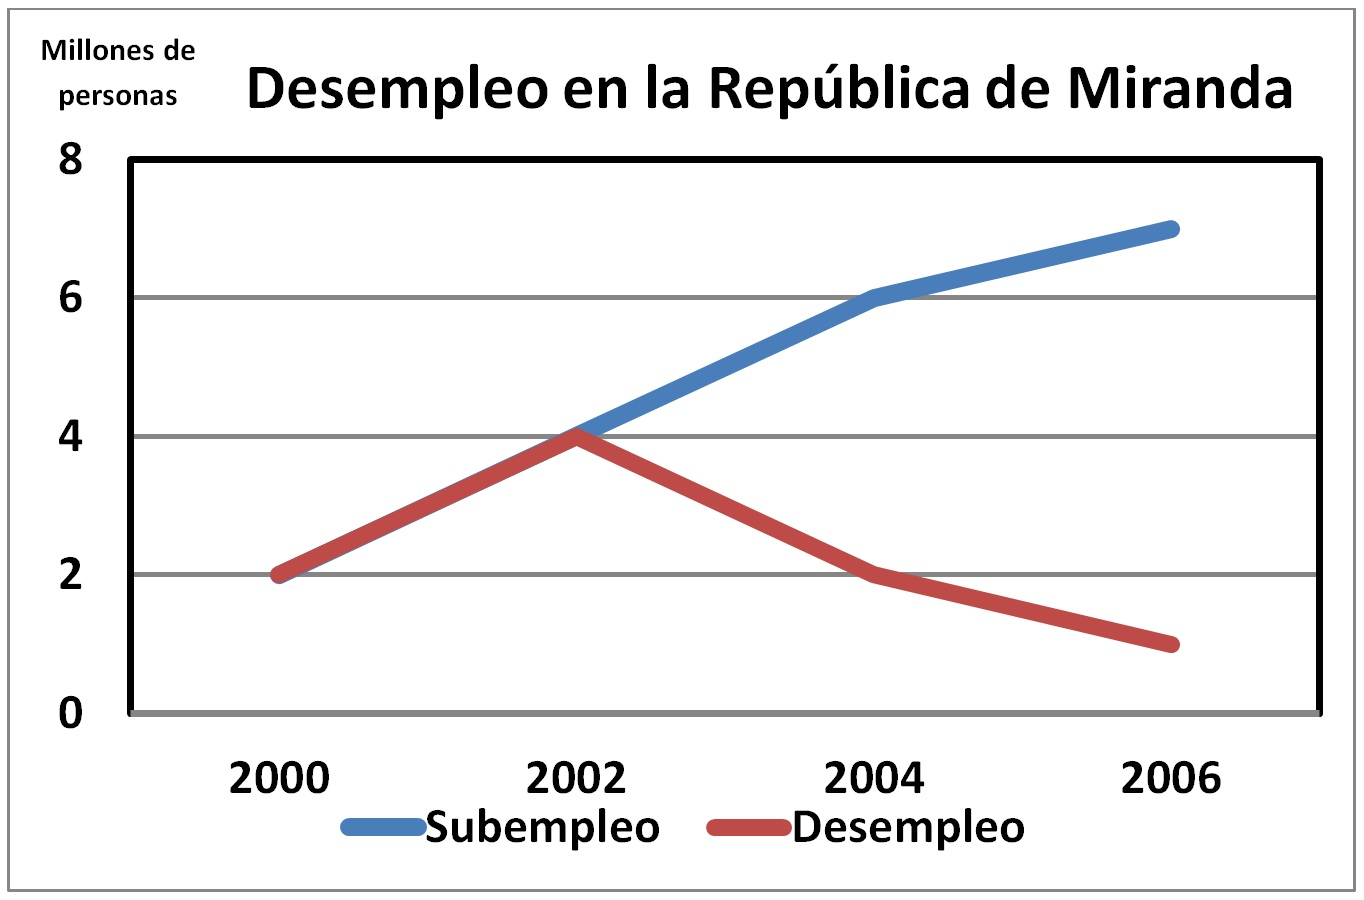
\includegraphics[width=0.45\textwidth]{sociii_img1.jpeg}

$\blacklozenge$ Se entiende por desempleo la situación de paro forzoso a la que es sometida aquella persona que teniendo las capacidades y el deseo de trabajar, no encuentra un empleo y por ende no percibe salario. \\

$\blacklozenge$ Se entiende por subempleo la situación de trabajo realizado sin suficiente regularidad o trabajo esporádico que se lleva a cabo cuando el trabajador no consigue una posición fija dentro del mercado laboral que le permita ocupar su disponibilidad temporal en un empleo estable. Dentro de esta categoría se encuentran los vendedores ambulantes y/o de economía informal.

\item De acuerdo con el gráfico 1, en la República de Miranda el subempleo:\label{sociii-23}


\begin{enumerate}[(A) ]
\item   Se toma en cuenta a partir del año 2000 registrando a dos millones de personas y para el año 2006 registraba siete millones de personas.
 \item  Se toma en cuenta a partir del año 2004 registrando a cuatro millones de personas y para el año 2006 registraba siete millones de personas.
\item Existía desde el año 2002 y registraba a dos millones de personas, pero recibía el nombre de desempleo.
\item Existía desde mucho antes de aparecer en la gráfica, pero se enmarcaba dentro de la categoría del desempleo.
\end{enumerate}
%%%%%%%%%%%%%%%%%%%%%%%%%%%%%

\item Se puede deducir que con relación a sus promesas de gobierno, el presidente Alberto Ubiria López:\label{sociii-24}


\begin{enumerate}[(A) ]
\item   Cumplió con lo prometido en tanto que la línea de desempleo disminuyó gradualmente hasta casi desaparecer por completo.
 \item  No cumplió con lo prometido debido a que nunca hubo una desaparición real del desempleo, sino una subsunción del mismo dentro de la categoría ``subempleo''.
\item Cumplió con lo prometido ya que en el 2002 recibió el país con cuatro millones de desempleados y lo entregó en el 2006 con tan sólo un millón.
\item No cumplió con lo prometido puesto que le faltó un millón de desempleados para lograr alcanzar sus metas propuestas.
\end{enumerate}
%%%%%%%%%%%%%%%%%%%%%%%%%%%%%

\item Se puede afirmar que para el 2006 la situación social y económica que atraviesa la República de Miranda es:\label{sociii-25}


\begin{enumerate}[(A)]
\item   Óptima ya que los niveles de desempleo han descendido de manera significativa.
 \item  Deficiente debido a que hay todavía un millón de personas que aún se encuentran sin trabajo.
\item Óptima puesto que de continuar la tendencia que registran las estadísticas, en menos de dos años se habría erradicado por completo el desempleo.
\item Deficiente, en tanto que se puede inferir que más de la mitad de la población se encuentra en la pobreza puesto que no existe una situación laboral estable que otorgue condiciones de trabajo y remuneración adecuados para la gran mayoría de la población. 
\end{enumerate}

%%%%%%%%%%%%%%%%%%%%%%%%%%%%%

%%%%%%%%%%%%%%%%%%%%%%%%%%%%%
\end{enumerate}
%%%%%%%%%%%%%%%%%%%%%%%%%%%%%5
